%%%%%%%%%%%%%%%%%%%%%%%%%%%%%%%%%%%%%%%%%
% Short Sectioned Assignment
% LaTeX Template
% Version 1.0 (5/5/12)
%
% This template has been downloaded from:
% http://www.LaTeXTemplates.com
%
% Original author:
% Frits Wenneker (http://www.howtotex.com)
%
% License:
% CC BY-NC-SA 3.0 (http://creativecommons.org/licenses/by-nc-sa/3.0/)
%
%%%%%%%%%%%%%%%%%%%%%%%%%%%%%%%%%%%%%%%%%

%----------------------------------------------------------------------------
%	PACKAGES AND OTHER DOCUMENT CONFIGURATIONS
%----------------------------------------------------------------------------

\documentclass[paper=a4, fontsize=11pt]{scrartcl} % A4 paper and 11pt font size

\usepackage[T1]{fontenc} % Use 8-bit encoding that has 256 glyphs
\usepackage{fourier} % Use the Adobe Utopia font for the document - comment this line to return to the LaTeX default
\usepackage[english]{babel} % English language/hyphenation
\usepackage{amsmath,amsfonts,amsthm} % Math packages

\usepackage{graphicx} % Used for including graphics
\usepackage{caption}
\usepackage{subcaption}

\usepackage{sectsty} % Allows customizing section commands
\allsectionsfont{\centering \normalfont\scshape} % Make all sections centered, the default font and small caps

\usepackage{fancyhdr} % Custom headers and footers
\usepackage{cite}
\bibliographystyle{plain}
\pagestyle{fancyplain} % Makes all pages in the document conform to the custom headers and footers
\fancyhead{} % No page header - if you want one, create it in the same way as the footers below
\fancyfoot[L]{} % Empty left footer
\fancyfoot[C]{} % Empty center footer
\fancyfoot[R]{\thepage} % Page numbering for right footer
\renewcommand{\headrulewidth}{0pt} % Remove header underlines
\renewcommand{\footrulewidth}{0pt} % Remove footer underlines
\setlength{\headheight}{13.6pt} % Customize the height of the header

\numberwithin{equation}{section} % Number equations within sections (i.e. 1.1, 1.2, 2.1, 2.2 instead of 1, 2, 3, 4)
\numberwithin{figure}{section} % Number figures within sections (i.e. 1.1, 1.2, 2.1, 2.2 instead of 1, 2, 3, 4)
\numberwithin{table}{section} % Number tables within sections (i.e. 1.1, 1.2, 2.1, 2.2 instead of 1, 2, 3, 4)

\setlength\parindent{0pt} % Removes all indentation from paragraphs - comment this line for an assignment with lots of text

%----------------------------------------------------------------------------
%	TITLE SECTION
%----------------------------------------------------------------------------

\newcommand{\horrule}[1]{\rule{\linewidth}{#1}} % Create horizontal rule command with 1 argument of height

\title{
\normalfont \normalsize
\textsc{King Abdullah University of Science and Technology\\
        Division of Mathematical and Computer Sciences and Engineering\\
        Design and Analysis of Algorithms} \\ [25pt] % Your university, school and/or department name(s)
\horrule{0.5pt} \\[0.4cm] % Thin top horizontal rule
\Large Midterm Project Report\\
\huge Diverse Approaches to Exact Pattern Matching
\horrule{2pt} \\[0.5cm] % Thick bottom horizontal rule
}

\author{Affara, Lama\\
        Almansour, Durrah\\
        Al-Shedivat, Maruan\\
        Chen, Gui\\
        Fujii, Chisato\\
        Rapakoulia, Trisevgeni}


\date{\normalsize\today} % Today's date or a custom date


\begin{document}
\begin{titlepage}
\maketitle
\thispagestyle{empty}
\clearpage
\end{titlepage}

%----------------------------------------------------------------------------
%    INTRODUCTION
%----------------------------------------------------------------------------

\section{Introduction}
Write introduction here...

\section{Boyre-Moore Algorithm}
Boyre Moore algorithm \cite{bm_fast} searches for all the occurrences of the pattern in the text. It is in some way similar to the naive search algorithm. Initially, it aligns the first character in P with the first character in T. The algorithm then compares characters between P and T sequentially from right to left. Once a mismatch occurs, a shift rule is applied thus moving the pattern by $s\ge 1$. The algorithm is basically divided into two stages: preprocessing and searching. There are two different preprocessing approaches in the literature: Bad Character Rule and Good Suffix Tree \cite{bm_tbc}. We decided to choose the Bad Character rule due to its simplicity and applicability to our dataset. In the following sections, we describe the two stages of the algorithm.

\subsection{Preprocessing Stage}
In the preprocessing stage, the algorithm makes use of the alphabet $\Sigma$ and the pattern P. A two dimensional table D is constructed by processing the pattern according to the available alphabet. D is of size $k\times|\Sigma|$ where for each mismatch index in P, the position of rightmost occurrence of a character in $\Sigma$ is stored. Figure \ref{fig:table} shows an example of the table stored by processing the pattern GCAGAGAG based on the DNA alphabet=\{A,C,G,T\}. Starting from the last row corresponding to a mismatch occurring at position i=k in P, i=8 for this example, the algorithm scans P to find the rightmost index of the given character. In the below example, the last occurrence of A before position 8 is 7, G is 6, C is 2, and T is 0. It is important to note here that if a character does not exist in the pattern, its position in the table is always 0. Now, the algorithm iterates from i=k to 1. If the mismatch occurs in position i-1, the algorithm updates only the value for the specific character placed in this position, A for this example, and all the other values remain the same as D[i,x]. The last occurrence of A before position 7 is 5, while G, C, and T stay the same.

\begin{figure}[h!]
\centering
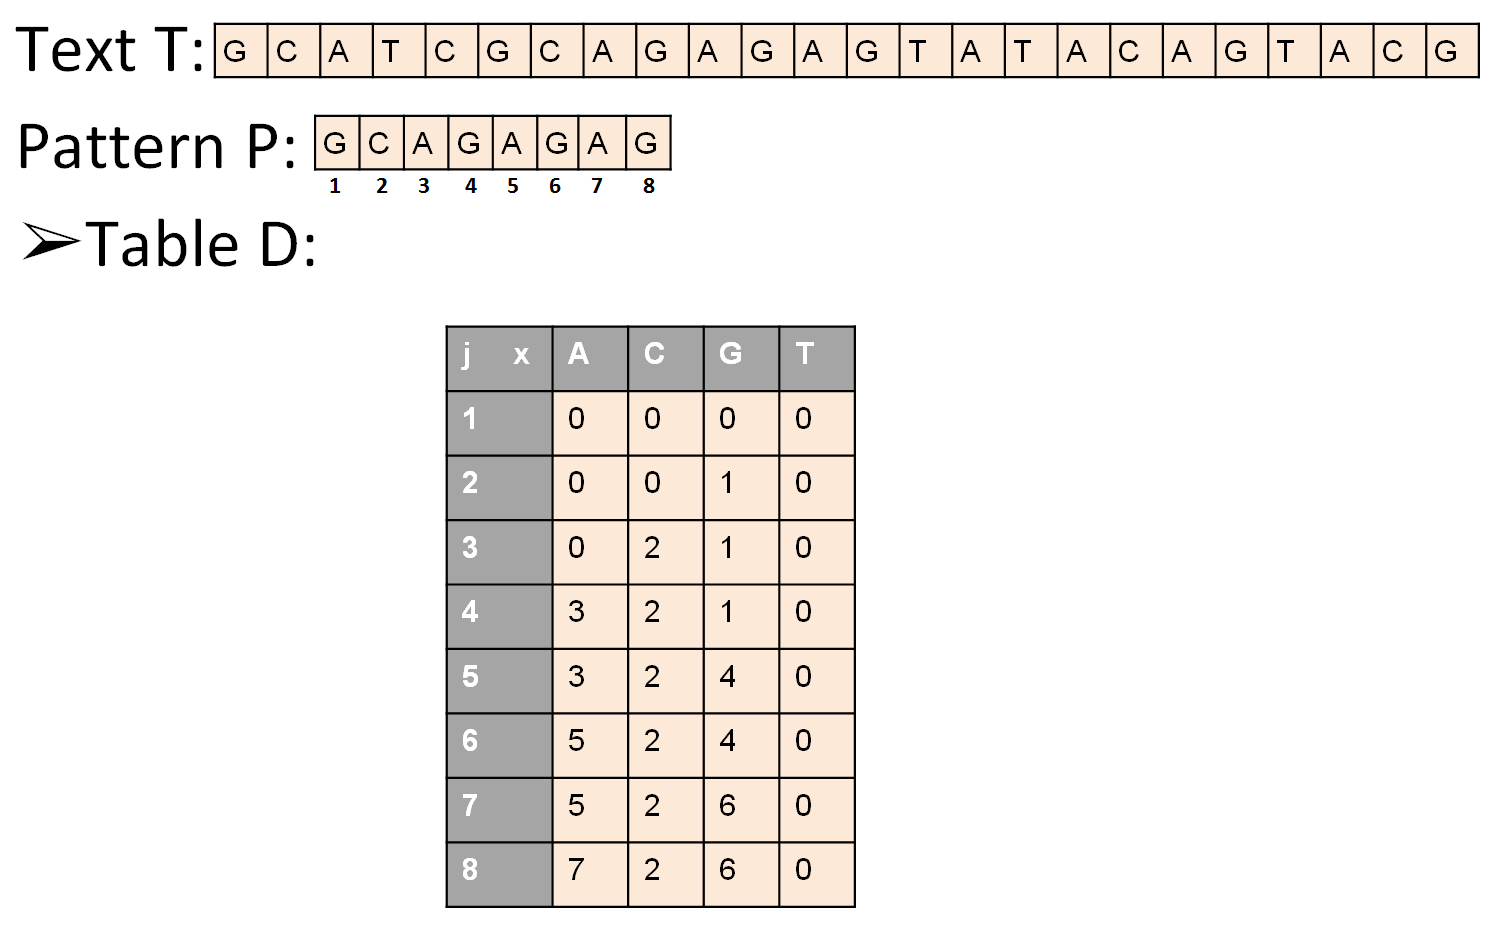
\includegraphics[width=0.8\textwidth]{figures/Example_Table.png}
\caption{Table of preprocessing phase}
\label{fig:table}
\end{figure}

\subsection{Searching Phase}
In the searching phase, the algorithm needs shift the pattern and sequentially match it with the aligned text. Starting from the rightmost character in P, the algorithm checks the aligned character in T. If the pair of characters are matching, it sequentially continues the check to the next left character. If a mismatch occurs at position j in P, the algorithm needs to shift P according to the mismatched character in the text. For example, if at position j, the text contains a character that is not found in P, the pattern should be shifted by j. However, if the mismatched character is found in P, the pattern should be shifted by j-i, where i corresponds to the rightmost occurrence of this character in P. The index i of the last occurrence is retrieved from table D and i=D[j,x] where x is the character in the text. Figure \ref{fig:search} shows the searching phase for the example shown in the previous section.

\begin{figure}[h!]
\centering
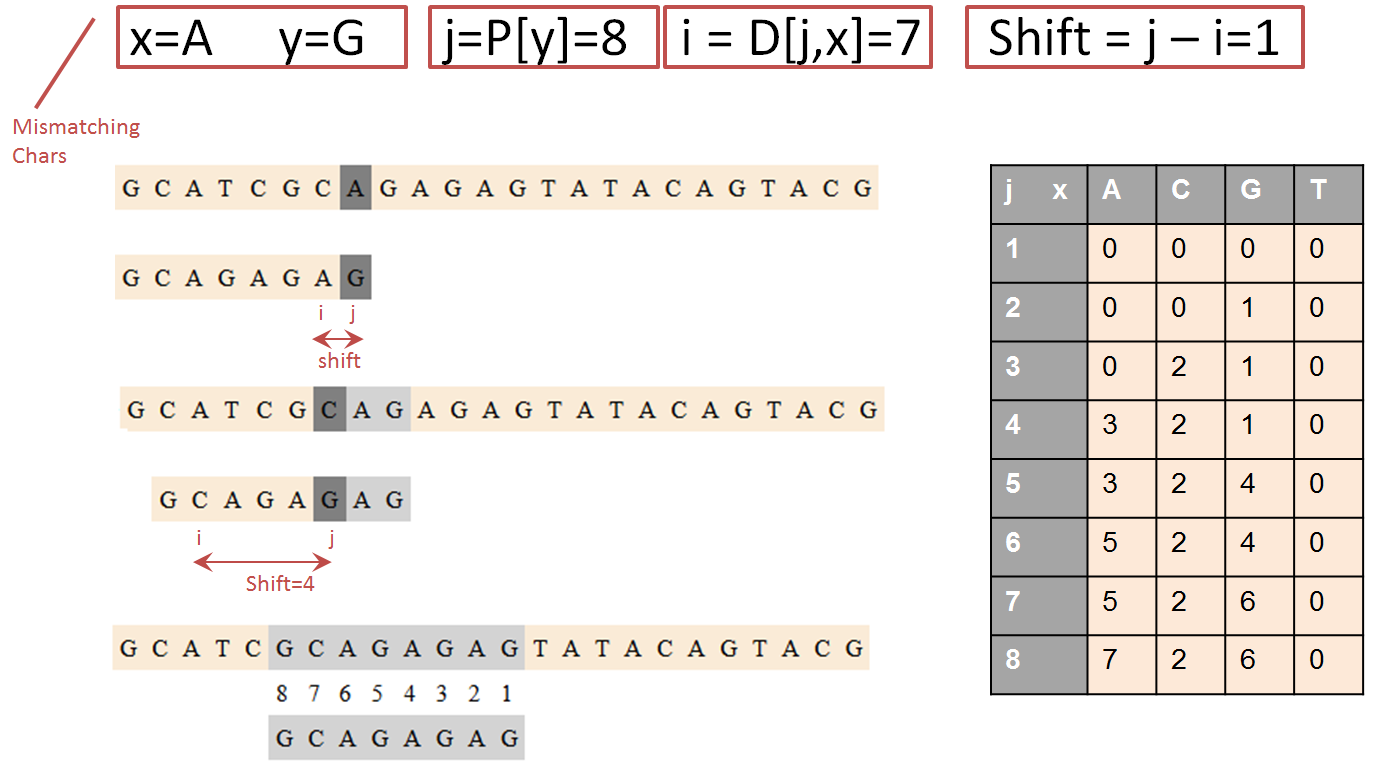
\includegraphics[width=0.8\textwidth]{figures/searching_phase.png}
\caption{Searching Phase}
\label{fig:search}
\end{figure}

\subsection{complexity}

\newpage
\section{Aho-Corasick Algorithm}
...

\newpage
\section{Suffix-tree Pattern Matching}
As the third part of our comparative study, we propose a pattern matching algorithm that relies on so called suffix tree data structure. Suffix tree is a well known data structure which is commonly used in industrial and scientific applications of pattern matching today. Being a concise representation of a text composed over a finite alphabet, suffix tree, or more general suffix automaton, is a common way to compress large amounts of textual information, and it is widely used also in databases. In our study, we will perform tests of suffix tree base pattern matching algorithm, and compare it against the aforementioned Boyer-More and Aho-Corasick algorithms, trying to get an insight on when should one chose either of these algorithms.\\

Below, we will introduce first \textit{suffix trie} -- an auxillary data structure -- which we will enhance into suffix tree. Along this way, we will show that suffix tree construction algorithm is a linear time algorithm, and that suffix tree is a linear-memory data structure, following the Ukkonen's construction algorithm~\cite{ukkonen1995online}. Suffix tree construction is the preprocessing step for the pattern matching algorithm. We also, describe how to use a suffix tree of a text to find out if a pattern matches the text, and show that procedure also takes pattern length linear time.

\subsection{Suffix Trie}
Being able to consider suffix tries, and following~\cite{ukkonen1995online}, we first introduce the notations. Let text T be a string $T = t_1 t_2 \dots t_n$ over an alphabet $\Sigma$; $T_i = t_i \dots t_n$ where $1 \leq i \leq n+1$ is a suffix of the text; lets also assume that $T_{n+1} = \varepsilon$, i.e. the empty suffix. Lets denote the set of all the suffixes of the text T by $\sigma(T)$. We name the following set of objects a \textit{suffix trie} of a text T

\begin{equation}
STrie(T) = \left\{Q \cup \{\perp\}, root, F, g, f \right\}
\end{equation}

which is a deterministic finite-state automaton (DFA) which has a tree-shaped transition graph representing the trie for $\sigma(T)$. It is augmented with so called \textit{suffix function} $f$ and with an auxiliary state $\perp$. In the presented notations, the set $Q$ is the set of all the states of $STrie(T)$, which could be put into one-to-one correspondence with the substrings of $T$, i.e. with all such $x$ that $T = a\ x\ v$, where $a$ is some prefix of $T$, and $v$ is some suffix of $T$. The initial state $root$ corresponds to the empty string $\varepsilon$, and the set of final states $F$ corresponds to all the suffixes $\sigma(T)$. Latin characters with bars will denote states; characters without bars will denote symbols or some sequences of symbols from the alphabet $\Sigma$; $\varepsilon$ will denote the empty string. Finally, the transition function $g$ is defined as $g(\bar{x}, a) = \bar{y}$ for all $\bar{x}, \bar{y} \in Q$ such that $y = xa$, where $a \in \Sigma$; $g(\perp, a) = root$ for all $a \in \Sigma$.\\

Now, the suffix function $f$ is defined for each state $\bar{x} \in Q$ as follows. If $\bar{x}$ is not $root$, then $x = az$ for some $a \in \Sigma$, and we set $f(\bar{x}) = \bar{z}$. If it is $root$, $f(root) = \perp$.\\

To online construct a suffix trie by reading a text $T$ from left to right symbol by symbol, we should notice the following. Suppose, we have already read some prefix of the text $T^i = t_1 \dots t_i$, and have already constructed a $STrie(T^i)$. Now, we read the next symbol $t_{i+1}$ from the text, and we need to add it to the structure and obtain $STrie(T^{i+1})$. One can notice, that all the new suffixes of $T^{i+1}$ could be obtained by concatenation of $t_{i+1}$ symbol to all the previous suffixes, i.e.

$$
\sigma(T^{i+1}) = \sigma(T^i)t_i \cup \varepsilon.
$$

By construction, the $STrie(T^i)$ accepts $\sigma(T^i)$, and we want to make it accept $\sigma(T^{i+1})$. For achieving this, we need to add $t_{i+1}$ transitions to all the $r \in F_i$ which don't have such. By doing this, we will properly update our transition function $g_i$ to $g_{i+1}$, and also we will get final states $F_i$ updated to $F_{i+1}$.\\

Also, we should update the suffix function $f_i$ up to $f_{i+1}$, such that for every $\bar{r} \in F_{i+1}$ the new suffix function $f_{i+1}(\bar{r}) = \bar{s}$, for which $r = as$, where $a \in \Sigma$. In order to do such an update, we notice that if $r \in F_i$, then there exists such $0 \le j \le i$, such that $r = f_i^j(\overline{t_1...t_i})$. This means that the suffix function connects all the final states in the $STrie(F_i)$ into a single path. We denote this path as the \textit{boundary path}.\\

So, the new suffix function $f_{i+1}$ should connect all the new final states $F_{i+1}$ and form a new boundary path. To achieve this, we can traverse all the $F_i$ states along the current boundary path, and make updates for every state on this path, adding a suffix link where it is necessary and adding a transition for a new symbol $t_{i+1}$ where it is necessary. Finally, it was shown in the original paper~\cite{ukkonen1995online} that while traversing the boundary path, if we encountered a state $\bar{z}$ that does have a transition $t_{i+1}$, there is no need to further continue traversing, since all of the further suffix successors of the state $\bar{z}$ are up-to-date and have both the right suffix links and also the right transitions $t_{i+1}$. Finally, the algorithm is going to be as it follows.

\begin{enumerate}
  \item Start from the state $\overline{t_1 t_2 \dots t_i}$ (the whole prefix preprocessed up to now).
  \item If there is no transition from the current state for symbol $t_{i+1}$, create a new state for such a transition. Memorize the newly created state.
  \item Follow the suffix link from the current state and again perform step (2).
  \item Create a suffix link from the last created state (on step 3) for transition on symbol $t_{i+1}$, to the state created right before that (on step 2).
  \item Repeat steps (2), (3) and (4) until we find that the current state has a transition on $t_{i+1}$.
\end{enumerate}

\begin{figure}[h!]
\centering
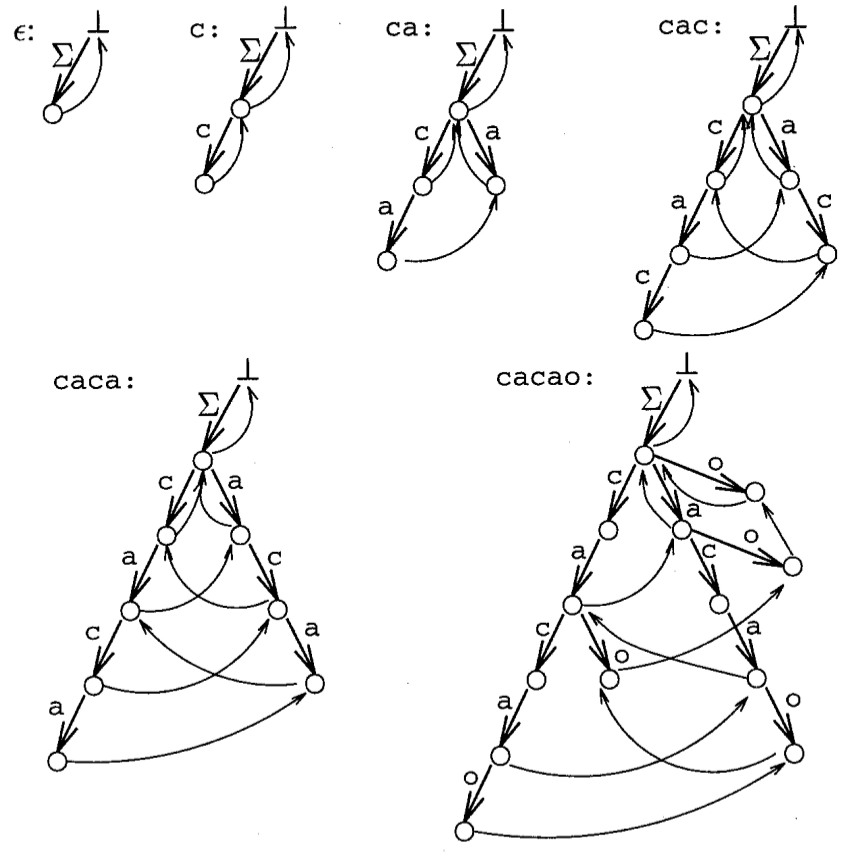
\includegraphics[width=0.8\textwidth]{figures/suffix-trie-eg.png}
\caption{An example of building a suffix trie for string "cacao". We start from the empty string, and the suffix tree augmented DFA consists of only $root$ and $\perp$ states at this stage. Then we add letter by letter the whole text. For each letter, we perform the above mentioned 5-step iterative algorithm to update the transition and suffix functions $g$ and $f$.}
\label{fig:siffix-trie}
\end{figure}

An example of how this algorithm works is presented in figure~\ref{fig:siffix-trie}. The algorithm obviously does a constant number of operations each of its iterations, and, in the worst case, it should visit all the nodes of the suffix trie $STrie(T^i)$ to update it up to $STrie(T^{i+1})$. So, it is optimal in the sense that its time complexity is proportional to the size of its end result $STrie(T)$. On the other hand, the size of $STrie(T)$ can be quadratic in $n = |T|$. To overcome this issue, we introduce the so called \textit{suffix tree} structure which is based on suffix trie, but is more concise and takes less memory and time to be built.

\subsection{Suffix Tree}

The suffix tree for the string $S$ of length $n$ is defined as a tree such that:
\begin{itemize}
  \item The tree has exactly $n$ leaves numbered from 1 to $n$.
  \item Except for the root, every internal node has at least two children.
  \item Each edge is labeled with a non-empty substring of $S$.
  \item No two edges starting out of a node can have string-labels beginning with the same character.
  \item  The string obtained by concatenating all the string-labels found on the path from the root to leaf $i$ spells out suffix $S[i..n]$, for $i$ from 1 to n.
\end{itemize}

\subsection{definitions of some notations}
For a text, let $T = t_1t_2...t_3$ be a string over an alphabet $\Sigma$. And each string $T_i = t_it_{i+1}...t_n$ where $1 \leq i \leq n+1$ is a $suffix$ of string $T$. In particular, $T_{n+1} = \varepsilon$ is the $empty$ suffix. We define suffix tree $STree(T)$ of $T$ to be a data structure that represents $STre(T)$ in space linear in the length $|T|$ of $T$. And we denote it as $STree(T) =$
$(Q^{'}$ 
$\cup$
$\{\bot\},$
$root, g^{'}, f^{'})$.Set $Q^{'}$ consists of all branching states (states from which there
are at least two transitions) and all leaves (states from which there are no transitions) of $STrie(T)$. By definition, $root$ is included in the branching states.
The other states of $STrie(T)$ (the states other than $root$ and $\bot$ from which
there is exactly one transition) are called implicit states as states of $STree(T)$; they
are not explicitly present in $STree(T)$. Here $\bot$ is an auxiliary state.

\bibliography{references}
\nocite{*}

\end{document}
